\chapter{Algebra}

%Potênciação

\section{Potênciação}
\subsection{Potência de Expoente Natural}

\newtheorem{definicao}{Definição}
\begin{definicao}
	Seja $a \in \mathbb{R} $ e $ n \in \mathbb{N}$. Potência de base $\textbf{a}$ e expoente $\textbf{n}$ é igual a:
\end{definicao}

\begin{equation*}
a^{n} = \overbrace{a \times a \times \cdots \times a  \times a}^n
\end{equation*}

\begin{equation*}
a^0 = 1 , a \neq 0
\end{equation*}


\textbf{Propriedades:}

Se $a$ e $b$ $ \in \mathbb{R}$ e  $n$ e $ m$ $ \in \mathbb{N}$, então valem as seguintes propriedades:
\begin{enumerate}
	\item $a^{m}a^{n} = a^{m+n}$
	\item $(a\cdot b)^n = a^n \cdot b^n$
	\item $\left(\dfrac{a}{b}\right)^n = \dfrac{a^n}{b^n} , b \neq 0$
	\item $(a^m)^n = a^{m\cdot n}$
\end{enumerate}
\textbf{Exemplos:}

\begin{itemize}

	\item $(-5)^0 = 1$
	\item $2^3 \cdot 2^2 = 2^{3+2} = 2^5 = 2\cdot 2\cdot 2\cdot 2\cdot 2 = 32$
	\item $(3\cdot 4)^2 = 3^2 \cdot 4^2 = 3\cdot 3 \cdot 4 \cdot 4 =9 \cdot 8 = 72$
	\item $\left(\dfrac{3}{2}\right)^2 = \dfrac{3^2}{2^3} = \dfrac{3\cdot 3}{2\cdot 2\cdot 2} =\dfrac{9}{8}$
	\item $(2^3)^2 = 2^{3 \cdot 2} = 2^6= 2\cdot 2\cdot 2\cdot 2\cdot 2 \cdot 2 = 64$
\end{itemize}


\subsection{Potência de Expoente Inteiro}

\newtheorem{definicao}{Definição}
\begin{definicao}
	Seja $a \in \mathbb{R}^* $ e $ n \in \mathbb{Z}$. Potência de base $\textbf{a}$ e expoente $\textbf{n}$ é igual a:	
\end{definicao}

$$ a^{-n} = \dfrac{1}{a^n}$$

\textbf{Propriedades:}

Se $a$ e $b$ $ \in \mathbb{R}^*$ e  $n$ e $ m$ $ \in \mathbb{Z}$, então valem as seguintes propriedades:

\begin{enumerate}

\item $\dfrac{a^m}{a^n} = a^{m-n}$
\item $a^{m}a^{n} = a^{m+n}$
\item $(a\cdot b)^n = a^n \cdot b^n$
\item $\left(\dfrac{a}{b}\right)^n = \dfrac{a^n}{b^n} $
\item $(a^m)^n = a^{m\cdot n}$

\end{enumerate}
\textbf{Exemplos:}

\begin{itemize}

	\item $(2)^{-2} = \dfrac{1}{2^2} = \dfrac{1}{4}$
	\item $ \dfrac{3^4}{3^2} = 3^{ 4-2} = 3^{2} = 9 $ 
	\item $ \dfrac{2^3}{2^5} = 2^{ 3-5} = 2^{-2} = \dfrac{1}{2^2} = \dfrac{1}{4}$
\end{itemize}

\subsection{Potência de Expoente Racional}

\newtheorem{definicao}{Definição}
\begin{definicao}
	Seja $a \in \mathbb{R}^*_+ $ e $ \dfrac{p}{q} \in \mathbb{Q} (p \in \mathbb{Z}$ e $ q \in \mathbb{N}^*_+)$. Potência de base $a$ e expoente $\dfrac{p}{q}$ é igual a:	
\end{definicao}

$$ a^{\frac{p}{q}} = \sqrt[q]{a^p} $$

\textbf{Propriedades:}

Se $a$ e $b$ $ \in \mathbb{R}^*_+$ e  $\dfrac{p}{q}$ e $\dfrac{r}{s} $ $ \in \mathbb{Z}$, então valem as seguintes propriedades:


\begin{enumerate}

\item $a^{\frac{p}{q}} \cdot a^{\frac{r}{s}} = a^{\frac{p}{q} + \frac{r}{s}}$

\item $\dfrac{a^{\frac{p}{q} }}{a^{\frac{r}{s} } } = a^{\frac{p}{q} - \frac{r}{s}}$

\item $(a\cdot b)^{\frac{p}{q}} = a^{\frac{p}{q}} \cdot b^{\frac{p}{q}}$

\item $\left(\dfrac{a}{b}\right)^{\frac{p}{q}} = \dfrac{a^{\frac{p}{q} }}{b^{\frac{p}{q} } }  $

\item $(a^{\frac{p}{q}})^{\frac{r}{s}} =  a^{\frac{p}{q} \cdot \frac{r}{s}   }$

\end{enumerate}


\textbf{Exemplos:}

\begin{itemize}

	\item $2^{\frac{1}{3}} \cdot 2^{\frac{2}{3}} = 2^{\frac{1}{3} + \frac{2}{3}} = 2^1 = 2$
	\item $\dfrac{3^{\frac{3}{5} }}{3^{\frac{1}{5} } } = 3^{\frac{3}{5} - \frac{1}{5}} = 3^{\frac{2}{5}}$
	\item $(5\cdot 4)^{\frac{1}{2}} = 5^{\frac{1}{2}} \cdot 4^{\frac{1}{2}} = \sqrt{5} \cdot \sqrt{4} = 2 \sqrt{5}$
	\item $\left(\dfrac{4}{3}\right)^{\frac{1}{2}} = \dfrac{4^{\frac{1}{2} }}{3^{\frac{1}{2} } } = \dfrac{\sqrt{4}}{\sqrt{3}} = \dfrac{2}{\sqrt{3}} = \dfrac{2}{\sqrt{3}} \cdot \dfrac{\sqrt{3}}{\sqrt{3}} = \dfrac{2\sqrt{3}}{3}  $
	\item $(6^{\frac{4}{3}})^{\frac{3}{2}} =  6^{\frac{4}{3} \cdot \frac{3}{2}   } = 6^{\frac{12}{6}}= 6^2 = 36$
\end{itemize}
\subsection{Potência de Expoente Irracional}

\newtheorem{definicao}{Definição}
\begin{definicao}
	Seja $a \in \mathbb{R} $ e $n$ um número irracional. Potência de base $a$ e expoente $n$ é  $a^n$.	
\end{definicao}

\textbf{Observações:}
\begin{itemize}
\item Se $a=0$ e $n$ é irracional e positivo, então:
$$ 0^n = 0$$ 
\item Se $a < 0 $ e $n$ é irracional e positivo, então $a^n$ não tem significado. Exemplos: $(-3)^{\sqrt{3}}$,$(-\sqrt{3})^{\sqrt{5}}$ e $(-9)^{\pi}$.
\item Se $n< 0$ então $0^n$ não tem significado.
\item Para as potências de expoente Irracional são válidas as propriedades anteriores.

\end{itemize}



\subsection{Potência de Expoente Real}
	
\newtheorem{definicao}{Definição}
\begin{definicao}
	Seja $a \in \mathbb{R}^*_+ $ e $ n \in \mathbb{R}$. Potência de base $a$ e expoente $n$ é  $a^n$.	
\end{definicao}

\textbf{Propriedades:}

Se $a$ e $b$ $ \in \mathbb{R}^*_+$ e  $n$ e $ m$ $ \in \mathbb{R}$, então valem as seguintes propriedades:

\begin{enumerate}
\item $ a^m \cdot a^n = a^{m+n}$
\item $\dfrac{a^m}{a^n} = a^{m-n}$
\item $(a\cdot b)^n = a^n \cdot b^n$
\item $\left(\dfrac{a}{b}\right)^n = \dfrac{a^n}{b^n} $
\item $(a^m)^n = a^{m\cdot n}$
\end{enumerate}
% Fim de Potênciação

\subsection{Radiciação}

Dados $a \in \mathbb{R}_+$ e $n \in \mathbb{N}, n \geq 1$, chama-se raiz n-ésima aritmética de $a$ o número real e não negativo $b$, tal que:
$$\sqrt[n]{a} = b \Leftrightarrow b^n = a$$


\textbf{Propriedades:}
Se $a$ e $b$ $ \in \mathbb{R}_+$ , $n$ e $ p$ $ \in \mathbb{N}$ e $m \in \mathbb{Z}$ então valem as seguintes propriedades:

\begin{enumerate}
\item $\sqrt[n]{a \cdot b} = \sqrt[n]{a} \cdot \sqrt[n]{b} $

\item $\sqrt[n]{\dfrac{a}{b}} = \dfrac{\sqrt[n]{a}}{\sqrt[n]{b}} ,\,\,\, b > 0$

\item $(\sqrt[n]{a})^m = \sqrt[n]{a^m}$

\item $\sqrt[n]{a^m} = \sqrt[n\cdot p]{a^{m\cdot p}}$

\item $\sqrt[p]{\sqrt[n]{a^m}} = \sqrt[p \cdot n]{a^m}$
\end{enumerate}

%Produtos Notaveis
\newpage
\section{Produtos Notáveis}

\subsection{Quadrado da Soma Entre Dois Termos}

	
	$$(a+b)^{2} = (a+b)(a+b) = a\cdot a + a\cdot b + b\cdot a + b\cdot b $$
	
	
	$$a^2+2ab+b^2$$
	
\begin{figure}[H]
	\centering
	
	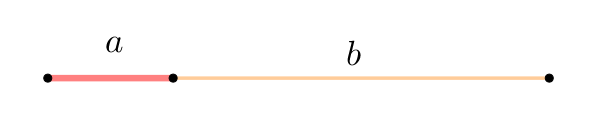
\includegraphics[scale=3.5]{imagens/soma-quadrado1.png}

\end{figure}

\begin{figure}[H]
	\centering
	
	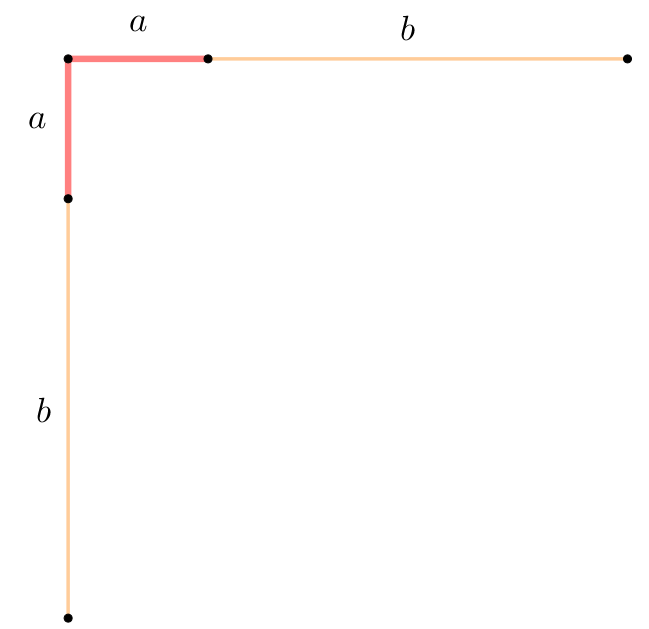
\includegraphics[scale=3.5]{imagens/soma-quadrado2.png}

\end{figure}
	
\begin{figure}[H]
	\centering
	
	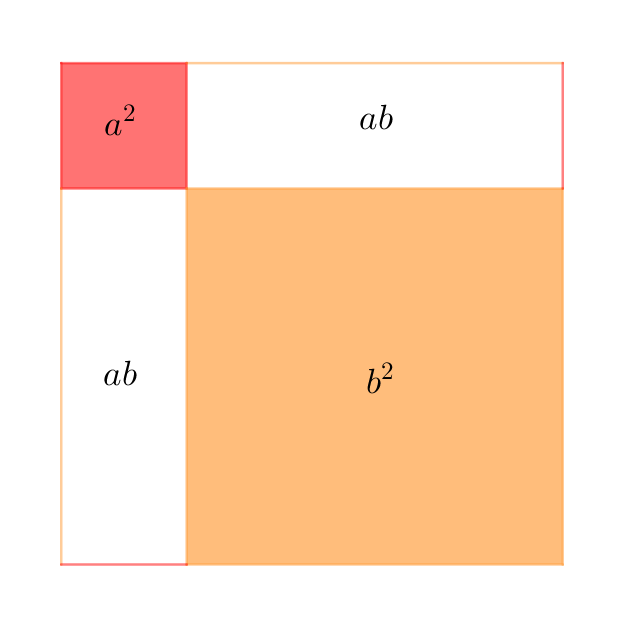
\includegraphics[scale=3.5]{imagens/soma-quadrado.png}

\end{figure}
	
\subsection{Quadrado da Diferença Entre dois Termos}

	$$(a-b)^{2} = (a-b)(a-b) = a\cdot a - a\cdot b - b\cdot a + b\cdot b $$
	
	$$a^2-2ab+b^2$$
	
\subsection{Diferença de Quadrados}

	$$(a+b)(a-b) = a\cdot a - a\cdot b + b\cdot a + b\cdot b $$
	
	$$a^{2}-b^{2}$$
	
\subsection{Cubo da Soma Entre Dois Termos}

	$$(a+b)^{3} = (a+b)(a+b)^{2} = (a+b)(a^{2}+2ab+b^{2}) = a\cdot a^{2} + 2a\cdot a \cdot b + a\cdot b^{2} + b\cdot a^{2} + 2\cdot a \cdot b\cdot b + b\cdot b^{2} $$
	
	$$a^{3} + 3a^{2}b + 3ab^{2}+b^{3}$$

\subsection{Cubo da Diferença Entre Dois Termos}

$$(a-b)^{3} = (a-b)(a-b)^{2} = (a-b)(a^{2}-2ab+b^{2}) = a a^{2} - a2ab + a\cdot b^{2} - b\cdot a^{2} + 2\cdot a \cdot b\cdot b - b\cdot b^{2} $$
	
	$$a^{3} - 3a^{2}b + 3ab^{2} - b^{3}$$
	
\section{Técnicas de Fatoração}


\subsection{Termo em Evidência}

	$$2x^{2}+2xy = 2x(x+y)$$
	
\subsection{Agrupamento}

	$$ax+ 5a + 5x + 25$$
	$$a(x+5)+5(x+5)$$
	$$(x+5)(a+5)$$
	
\subsection{Quadrado perfeito}

	$$x^{2} + 8x +16 = x^{2}+2\cdot 4\cdot x + 4^{2} = (x+4)^{2}$$
	
	
\subsection{Diferença de Quadrados}

	$$x^{2} - 25 = x^{2} - 5^{2} = (x+5)(x-5)$$
	
\subsection{Soma de Dois Cubos}

	$$x^{3}+y^{3} = (x+y)(x^{2} - xy + y^{2})$$
	
\subsection{Diferença de Dois Cubos}

	$$x^{3} - y^{3} = (x-y)(x^{2} + xy + y^{2})$$
	
\subsection{Fatorações Sucessivas}

	$$3x^{2} - 75 = 3x^{2} - 3\cdot 25 = 3(x^{2} - 25) = 3(x^{2} - 5^{2}) = 3(x+5)(x-5)$$
	